%% Template for MLP Coursework 2 / 6 November 2017 

%% Based on  LaTeX template for ICML 2017 - example_paper.tex at 
%%  https://2017.icml.cc/Conferences/2017/StyleAuthorInstructions

\documentclass{article}
\usepackage[T1]{fontenc}
\usepackage{amssymb,amsmath}
\usepackage{txfonts}
\usepackage{microtype}

% For figures
\usepackage{graphicx}
\usepackage{subfigure} 

% For citations
\usepackage{natbib}

% For algorithms
\usepackage{algorithm}
\usepackage{algorithmic}

% the hyperref package is used to produce hyperlinks in the
% resulting PDF.  If this breaks your system, please commend out the
% following usepackage line and replace \usepackage{mlp2017} with
% \usepackage[nohyperref]{mlp2017} below.
\usepackage{hyperref}
\usepackage{url}
\urlstyle{same}

% Packages hyperref and algorithmic misbehave sometimes.  We can fix
% this with the following command.
\newcommand{\theHalgorithm}{\arabic{algorithm}}


% Set up MLP coursework style (based on ICML style)
\usepackage{mlp2018}
\mlptitlerunning{MLP Coursework 1 (\studentNumber)}
\bibliographystyle{icml2017}


\DeclareMathOperator{\softmax}{softmax}
\DeclareMathOperator{\sigmoid}{sigmoid}
\DeclareMathOperator{\sgn}{sgn}
\DeclareMathOperator{\relu}{relu}
\DeclareMathOperator{\lrelu}{lrelu}
\DeclareMathOperator{\elu}{elu}
\DeclareMathOperator{\selu}{selu}
\DeclareMathOperator{\maxout}{maxout}

\usepackage{url}
\usepackage{graphicx} 
\usepackage{float}

%% You probably do not need to change anything above this comment

%% REPLACE this with your student number
\def\studentNumber{sXXXXXXX}

\begin{document} 

\twocolumn[
\mlptitle{MLP Coursework 2: Exploring Convolutional Networks}

\centerline{\studentNumber}

\vskip 7mm
]

\begin{abstract} 
The abstract should be a few sentences (100--200 words) long,  providing a concise summary of the contents of your report including the key research question(s) addressed, the methods explored, the data used, and the findings of the experiments.
\end{abstract} 

\section{Introduction}
\label{sec:intro}
This document provides a template for the MLP coursework 2 report.  This template structures the report into sections, which you are recommended to use, but can change if you wish.  If you want to use subsections within a section that is fine, but please do not use any deeper structuring. In this template the text in each section will include an outline of what you should include in each section, along with some practical LaTeX examples (for example figures, tables, algorithms).  Your document should be no longer than \textbf{six pages},  with an additional page (or more!) allowed for references.

The introduction should place your work in context, giving the overall motivation for the work, and clearly outlining the objectives of the work and the research questions you have explored -- in this case the implementation of convolutional networks and the exploration of how context is handled in convolutional networks.  Most of the report will be to do with part 2.  

This section should also include a concise description of the Balanced EMNIST task and  data -- be precise: for example state the size of the training, validation, and test sets.  

\section{Implementing convolutional networks} 

Traditional neural networks use matrix multiplication to establish the connection between input and output, while convolutional neural networks use convolution to describe the relationship between input and output.
A convolutional neural network generally consists of five kinds of layers: input layers,convolutional layers, detector stage, pooling layers and  full connected layers. Below we will focus on the convolutional layers and the pooling layers.

\subsection{Convolutional layer}

Compared to the traditional fully connected layer, the convolution layer is faster and requires less storage space because the convolution layer has two features of sparse interactions and parameter sharing.

\textbf{sparse interactions}\\
Traditional neural networks have a relationship between each input and each output, whereas an output of a convolutional network only has a relationship with a portion of the input.This feature is achieved by making the size of the kernel much smaller than the size of the input.\cite{deeplearning2016}.

\textbf{parameter sharing}\\
In a model, the same set of parameters is used multiple times in multiple functions.\cite{deeplearning2016}.
This means that pixels in different positions of the input will operate with the same kernel, learning the same set of parameters.

Taking our experiment as an example, our input is a 28 $\times$ 28 pixel image, and we only need a 3 $\times$ 3 kernel which is used to detect some small meaningful features in the image. The output is a 26 $\times$ 26 feature map(padding = 0, stride = 1).

\begin{table}[H]
  \centering
%  \caption{compare convolutional layer with full connected layer}
    \begin{tabular}{lll}
          & convolutional layer & full connected layer \\
    parameters & 3 $\times$ 3 + 1  & 28 $\times$ 28 $\times$ 100  \\
    hidden units & 26 $\times$ 26 & 100 \\
    connections & 26 $\times$ 26 $\times$ 3 $\times$ 3 & 28 $\times$ 28 $\times$ 100 \\
    \end{tabular}%
  \label{clayertable1}
\end{table}%
The number of parameters and connections in the convolutional layer is much smaller than the fully connected layer. And if the stride is increased, the effect will be more significant.This not only reduces storage requirements, but also reduces the amount of computation.
\subsection{pooling layer}
Normally, the convolution layer will pass the result to the detector stage (for example Relu) after processing, after which the pooling layer will further adjust the data and pass to next convolution layer.
The pooling layer has several very important functions\\

\textbf{invariance}\\
When the input of this layer undergoes a small amount of translation and rotation, the output obtained will not change after being processed by the pooling function\cite{deeplearning2016}.This means that we are more concerned with the existence of a feature rather than the location of the specific feature.This is a very useful feature.For example,For the mnist dataset, because of the handwriting reason, the different number "1" may be in the left-hand side, the right-hand position, or a small amount of rotation relative to the standard one. But after the pooling function, the "1" they showed was consistent.

\textbf{Reduce the input of next layer}\\
Each area entered will perform pooling functions (such as max pooling, average pooling, etc.) to further extract features, reduce input dimensions, and output smaller dimensions.
\begin{figure}[H] %H为当前位置,!htb为忽略美学标准,htbp为浮动图形
		\centering %图片居中
		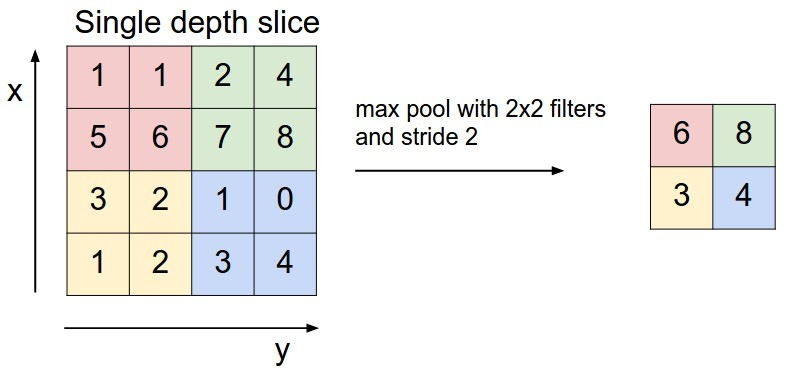
\includegraphics[width=0.4\textwidth]{./pic/part1/maxpool.jpeg} %插入图片,[]中设置图片大小,{}中是图片文件名
		\caption{Maxpooling} %最终文档中希望显示的图片标题
		\label{Fig.main2} %用于文内引用的标签
		\cite{cs231n}
\end{figure}
This image shows that After max pooling, the input has been reduced from 4 $\times$ 4 to 2 $\times$ 2.
It is precisely because the pooling function further extracts features that there are two effective functions. One is to enhance the fitting. Because the features are more obvious, the model is easier to learn the main features, and the generalization ability is strengthened. The other is to prevent over-fitting, because during the extraction process, only the main features are retained, and some relatively weak features are lost, which can prevent the model from over-fitting.

\subsection{Implementation}

\textbf{Convolutional layer}\\
The method I use is convolve2d. With this convolution method, we only need to find the input location and kernels, and then perform the convolution calculation. Of course, we also need to consider the input channel and output channel.
\begin{figure}[H] %H为当前位置,!htb为忽略美学标准,htbp为浮动图形
	\centering %图片居中
	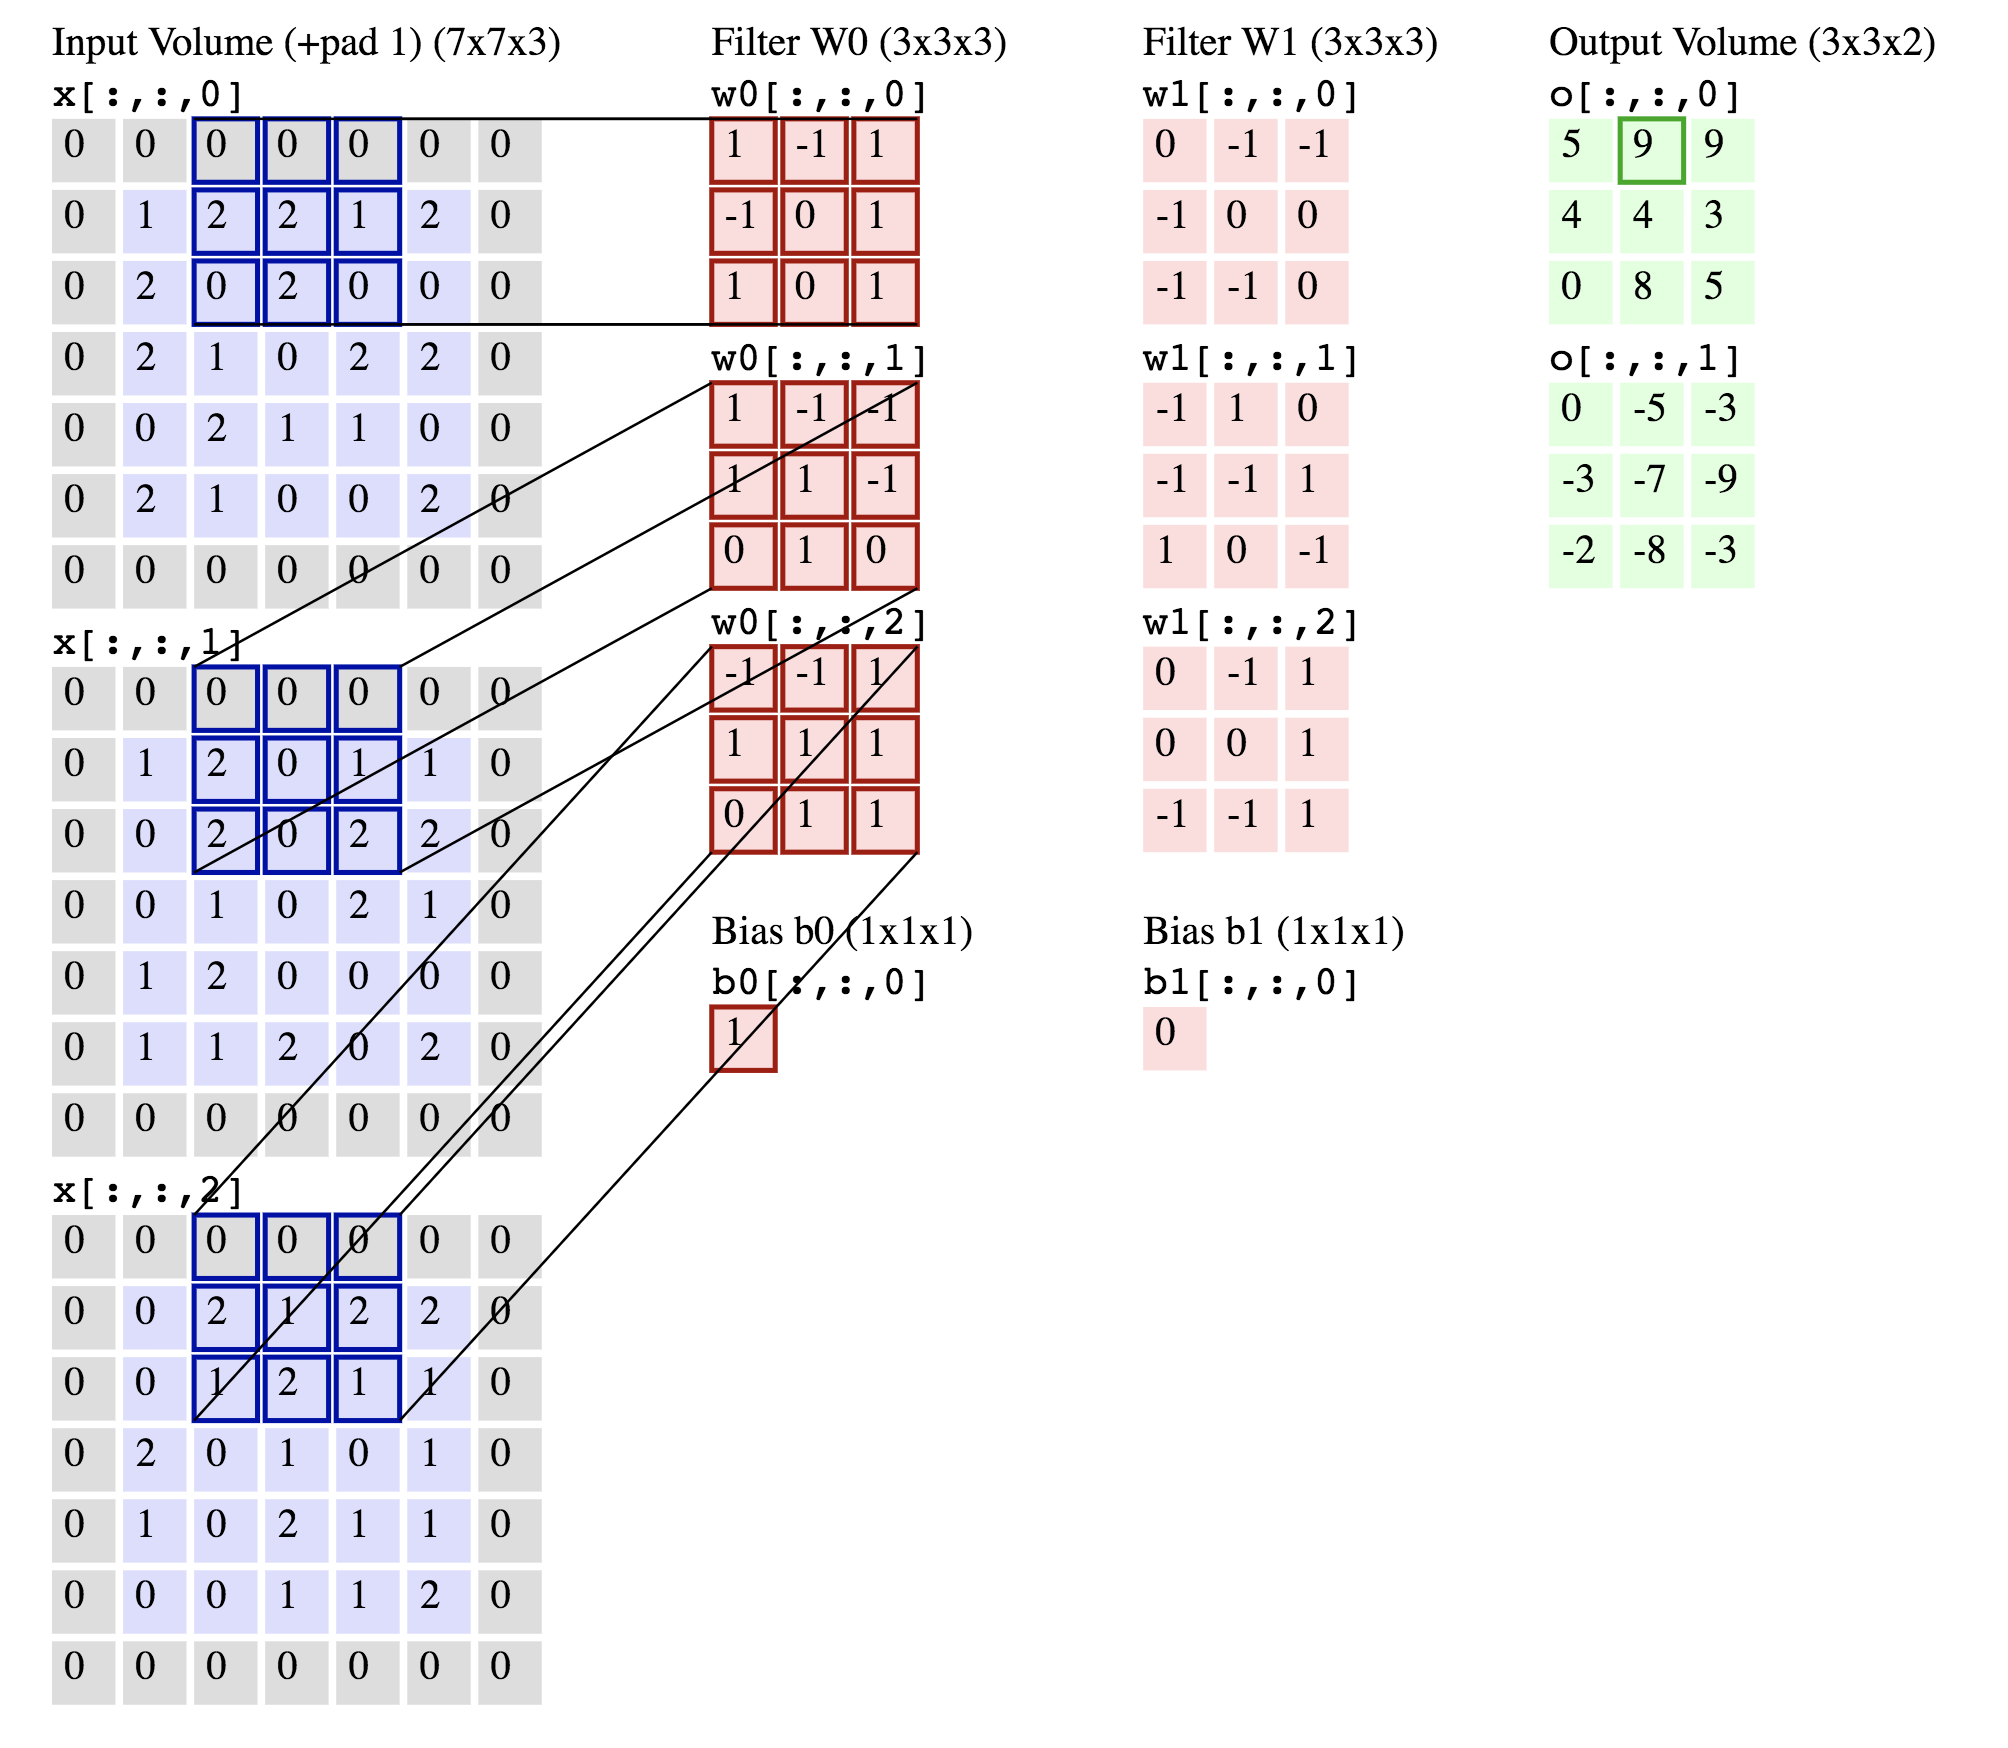
\includegraphics[width=0.45\textwidth]{./pic/part1/cnlayerImp.png} %插入图片,[]中设置图片大小,{}中是图片文件名
	\caption{convoluation layer implementation} %最终文档中希望显示的图片标题
	\label{Fig.main2} %用于文内引用的标签
	\cite{cs231n}
\end{figure}
The same is true for my implementation. I create 3 loops corresponding to batch  size, input channel and output channel, then find the input matrix of the image and the kernel matrix for convolution. After that, because there are multiple channels, I need to accumulate.For backpropagation, the implementation is similar, but it becomes the output weight and the kernel performs the convolution operation, but the kernel needs to be transposed first. For the grads wrt params function, we need input and output weights for convolution, but we need to transpose the inputs matrix first.\\

\textbf{Pooling layer}\\
The pooling algorithm I implemented is max pooling.
\begin{figure}[H] %H为当前位置,!htb为忽略美学标准,htbp为浮动图形
	\centering %图片居中
	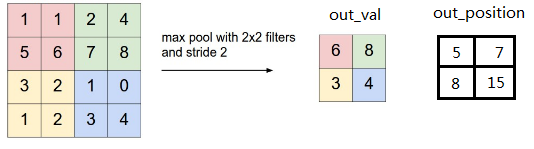
\includegraphics[width=0.5\textwidth]{./pic/part1/mpImpfprop.png} %插入图片,[]中设置图片大小,{}中是图片文件名
	\caption{maxpooling forward propagation implementation} %最终文档中希望显示的图片标题
	\label{Fig.main2} %用于文内引用的标签
\end{figure}
For the following figure, the input data X is 4*4, the sampling core size is 2, stride is 2, and no padding. The input data size is similar to the convolutional layer calculation method (input-width+2$\times$pad-pool-size)/stride+1. Forward propagation not only calculates the maximum value in the pool area, but also records the position in the input data of the maximum value. The purpose is to pass the gradient value to the position where the corresponding maximum value is in the backpropagation.
So for the backpropagation,It is known by forwardpropagation that the gradient value corresponds to the maximum position of the output of the previous layer. The specific process is as follows:
\begin{figure}[H] %H为当前位置,!htb为忽略美学标准,htbp为浮动图形
	\centering %图片居中
	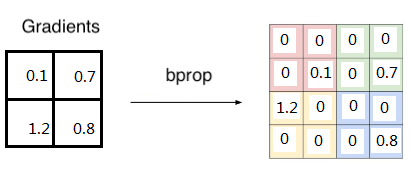
\includegraphics[width=0.5\textwidth]{./pic/part1/mpImpBprop.png} %插入图片,[]中设置图片大小,{}中是图片文件名
	\caption{maxpooling backpropagation implementation} %最终文档中希望显示的图片标题
	\label{Fig.main2} %用于文内引用的标签
\end{figure}
\subsection{Different approaches to implementing convolutional layers}
Here we will discuss three algorithms which are used for convolutional layer calculations, namely, correlate2d, im2col and Fast Fourier Transforms.
Correlate2d is a traditional convolution algorithm, although there is no advantage in speed compared to the other two, but in storage, no additional storage requirements are required.

Im2col is the multiplication of the convolution calculation into two matrices: 1. Convert the image into a matrix using im2col; 2. Convert the convolution kernel into a matrix using im2col; 3. Multiply the matrix from the first two steps.If stride < kernel size, then a large number of repeating pixels will be included in the matrix after the conversion, which is a big drain for memory. This is an obvious disadvantage of im2col for convolution operations, but this shortcoming is negligible compared to the speed gain of multiplying large matrices.

The process using the Fourier algorithm is such that the convolution in the time domain is equal to the product in the frequency domain, so after transforming our image (input) and kernel into the frequency domain, we multiply them directly, and then Transform back to the time domain. This completes the convolution operation.Because the size of a general convolution kernel is smaller than the image, we need to extend our kernel to match the size of the image.So you need to use the loop fill method to expand the convolution kernel so that the last two signals can be the same size when multiplied.The advantage of convolution calculations in the above manner is obvious - greatly reducing the amount of computation for direct convolution operations in the time domain.The disadvantages are also very obvious, because in a general convolutional neural network, the kernel is much smaller than the input, so additional memory space is needed when converting the kernel. Fourier's multiplication calculation is more complicated.

In summary, although im2col requires more memory space, it has an advantage in speed. Traditional convolution operations do not require extra memory space, but there is no advantage in speed. The memory space required by the Fourier algorithm and the efficiency of the algorithm are closely related to the size of kernal. When the core is large, the memory requirement is small, and the algorithm is efficient, and vice versa.

\section{Context in convolutional networks}
This section should introduce the main part of the report which is to do with exploring different ways of modelling context in convolutional networks.  This section should present, in your own words, the different approaches you have adopted, explaining how they work and what the key differences between them are.  You may reference the literature where appropriate.   You should also outline the key research questions that you have addressed in this work.

If you present algorithms, you can use the \verb+algorithm+ and \verb+algorithmic+ environments to format pseudocode (for instance, Algorithm~\ref{alg:example}). These require the corresponding style files, \verb+algorithm.sty+ and \verb+algorithmic.sty+ which are supplied with this package. 

\begin{algorithm}[ht]
\begin{algorithmic}
   \STATE {\bfseries Input:} data $x_i$, size $m$
   \REPEAT
   \STATE Initialize $noChange = true$.
   \FOR{$i=1$ {\bfseries to} $m-1$}
   \IF{$x_i > x_{i+1}$} 
   \STATE Swap $x_i$ and $x_{i+1}$
   \STATE $noChange = false$
   \ENDIF
   \ENDFOR
   \UNTIL{$noChange$ is $true$}
\end{algorithmic}
  \caption{Bubble Sort}
  \label{alg:example}
\end{algorithm}


\section{Experiments}
This section should cover the experiments carried out. For each experiment, make clear why it was carried out, what you were trying to discover. Describe carefully how you carried out the experiments, mentioning and justifying any hyperparameter settings.  As always, your aim is to give enough information so that someone else (e.g. another MLP group) could reproduce the experiment precisely.  Note that it is interesting to consider both accuracy / generalisation and runtime / memory requirements.

Present the experimental results clearly and concisely.  Usually a result is in comparison or contrast to a result from another approach please make sure that these comparisons/contrasts are clearly presented.  You can facilitate comparisons either using graphs with multiple curves or (if appropriate, e.g. for accuracies) a results table. You need to avoid having too many figures, poorly labelled graphs, and graphs which should be comparable but which use different axis scales. A good presentation will enable the reader to compare trends in the same graph -- each graph should summarise the results relating to a particular research (sub)question.

There is no need to include code or specific details about the compute environment.

As before, your experimental sections should include graphs (for instance, figure~\ref{fig:sample-graph}) and/or tables (for instance, table~\ref{tab:sample-table})\footnote{These examples were taken from the ICML template paper.}, using the \verb+figure+ and \verb+table+ environments, in which you use \verb+\includegraphics+ to include an image (pdf, png, or jpg formats).  Please export graphs as 
\href{https://en.wikipedia.org/wiki/Vector_graphics}{vector graphics}
rather than \href{https://en.wikipedia.org/wiki/Raster_graphics}{raster
files} as this will make sure all detail in the plot is visible.
Matplotlib supports saving high quality figures in a wide range of
common image formats using the
\href{http://matplotlib.org/api/pyplot_api.html\#matplotlib.pyplot.savefig}{\texttt{savefig}}
function. \textbf{You should use \texttt{savefig} rather than copying
the screen-resolution raster images outputted in the notebook.} An
example of using \texttt{savefig} to save a figure as a PDF file (which
can be included as graphics in a \LaTeX document is given in the coursework document.

If you need a figure or table to stretch across two columns use the \verb+figure*+ or \verb+table*+ environment instead of the \verb+figure+ or \verb+table+ environment.  Use the \verb+subfigure+ environment if you want to include multiple graphics in a single figure.

\begin{figure}[tb]
\vskip 5mm
\begin{center}
\centerline{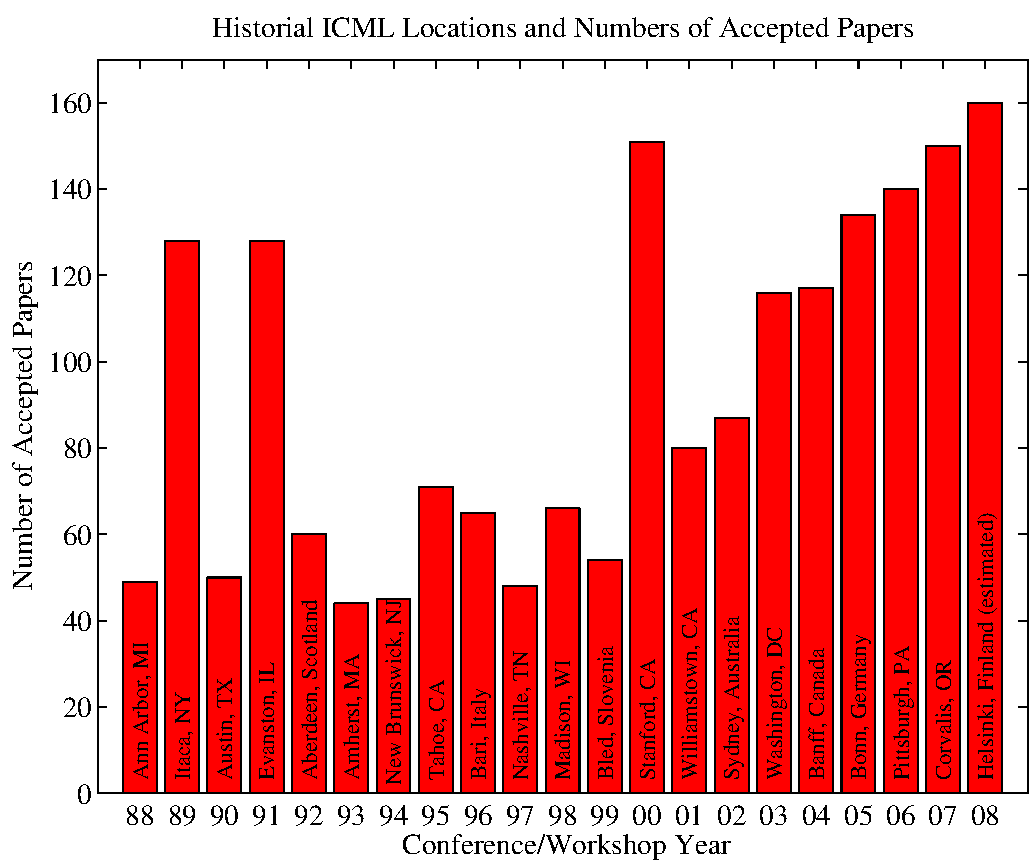
\includegraphics[width=\columnwidth]{icml_numpapers}}
\caption{Historical locations and number of accepted papers for International
  Machine Learning Conferences (ICML 1993 -- ICML 2008) and
  International Workshops on Machine Learning (ML 1988 -- ML
  1992). At the time this figure was produced, the number of
  accepted papers for ICML 2008 was unknown and instead estimated.}
\label{fig:sample-graph}
\end{center}
\vskip -5mm
\end{figure} 

\begin{table}[tb]
\vskip 3mm
\begin{center}
\begin{small}
\begin{sc}
\begin{tabular}{lcccr}
\hline
\abovespace\belowspace
Data set & Naive & Flexible & Better? \\
\hline
\abovespace
Breast    & 95.9$\pm$ 0.2& 96.7$\pm$ 0.2& $\surd$ \\
Cleveland & 83.3$\pm$ 0.6& 80.0$\pm$ 0.6& $\times$\\
Glass2    & 61.9$\pm$ 1.4& 83.8$\pm$ 0.7& $\surd$ \\
Credit    & 74.8$\pm$ 0.5& 78.3$\pm$ 0.6&         \\
Horse     & 73.3$\pm$ 0.9& 69.7$\pm$ 1.0& $\times$\\
Meta      & 67.1$\pm$ 0.6& 76.5$\pm$ 0.5& $\surd$ \\
Pima      & 75.1$\pm$ 0.6& 73.9$\pm$ 0.5&         \\
\belowspace
Vehicle   & 44.9$\pm$ 0.6& 61.5$\pm$ 0.4& $\surd$ \\
\hline
\end{tabular}
\end{sc}
\end{small}
\caption{Classification accuracies for naive Bayes and flexible 
Bayes on various data sets.}
\label{tab:sample-table}
\end{center}
\vskip -3mm
\end{table}






\section{Discussion}
Your discussion should interpret the results, both in terms of summarising the outcomes of a particular experiment, and attempting to relate to the research question(s) which motivated the experiments . A good report would have some analysis, resulting in an understanding of why particular results are observed, perhaps with reference to the literature. Use bibtex to organise your references -- in this case the references are in the file \verb+example-refs.bib+.  Here is a an example reference \citep{langley00}.  

A good report will relate the results to  published work which can help to give a better understanding of your work -- related approaches, other work on the same data, ideas for future work. 



% \textbf{Conclusions:}  


\section{Conclusions}
\label{sec:concl}
The conclusions section should concisely summarise what you have learned from the experiments you carried out, and relate the findings of your work to the  research questions you posed at the start.   It is good if the conclusion from one experiment influenced what you did in later experiments -- your aim is to learn from your experiments.   

A good conclusions section would also include a further work discussion, building on work done so far, and referencing the literature where appropriate.

\bibliography{example-refs}

\end{document} 

